\subsection{Statisk temperatur i vägg}


De ekvationer som beskriver värmeflöde är fouriers värmeekvation
\eqref{eq:staticwallmethod:fourier} samt värmeledningsekvationen
\eqref{eq:staticwallmethod:heat}. \\I dessa så är
$k$ värmeledningsförmågan i $\mbox{W}\mbox{m}^{-2}\mbox{K}^{-1}$ och
$\alpha$ är termisk diffusivitet i $\mbox{m}^2\mbox{s}^{-1}$. \cite{physicshandbook}

Då vi har statiskt värmeflöde
så kommer temperaturderivatan med avseende på tiden att vara noll.
Detta innebär att värmeledningsekvationen övergår till Laplaces ekvation
$\Delta{}T = 0$. I en dimension så blir detta $d^2T/dx^2 = 0$ vilket innebär
att lösningen blir ett polynom av första ordningen.  

\begin{equation}
\label{eq:staticwallmethod:fourier}
q_x = -k\frac{dT}{dx}
\end{equation}

\begin{equation}
\label{eq:staticwallmethod:heat}
\frac{\partial{}T}{\partial{}t} = \alpha\Delta{}T
\end{equation}

\begin{figure}
\centering
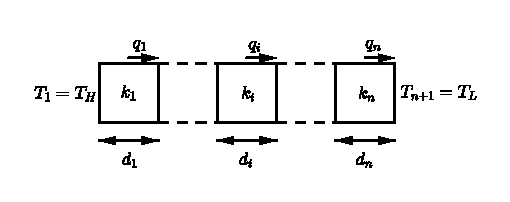
\includegraphics{images/wall.eps}
\caption{Schematisk bild över en vägg som består av $n$ olika element med olika
längd och värmeledningskapacitet.}\label{fig:staticwallmethod:wall}
\end{figure}

\noindent
Vi vill nu beskriva det statiska värmeflödet genom en vägg som består
av flera olika material. De enda värmekällorna som påverkar staven
är att vi har en isoterm $T = T_H$ på ena sidan av staven
samt en isoterm $T = T_L$ på andra sidan av staven.

För att göra beräkningarna enklare så
approximerar vi att väggen är oändligt lång. Detta innebär att vi kan räkna
på ekvationen i en dimension. En schematisk bild över en stav som består av
$n$ olika material kan ses i figur \ref{fig:staticwallmethod:wall}.
Vi benämner nu värmeledningsförmågan i materialen som $k_i$ samt längden
på elementen som $L_i$. Vi använder nu Fouriers ekvation för värmeledning för
att teckna värmeflödet och temperaturerna $T_j$, $j=0,1,..,n$ i punkterna
mellan de olika delarna av staven med randvillkoren $T_0 = T_H$ samt
$T_n = T_L$.

För varje del av staven så kan vi sätta upp ekvationer från Fouriers ekvation
för värmeflöde. Vi får flöde in i en del enligt \eqref{eq:staticwallmethod:rod} och
flödet ut genom staven blir detsamma ty temperaturen är konstant. Dessa två
ekvationer låter oss att teckna ett ekvationssystem för varje del av staven
enligt \eqref{eq:staticwalltheory:rodmatrix}.

\begin{equation}
\label{eq:staticwallmethod:rod}
Q = -k\frac{T_{2}-T_{1}}{L}
\end{equation}


\begin{equation}
\label{eq:staticwalltheory:rodmatrix}
\begin{pmatrix}
Q \\
-Q
\end{pmatrix} = 
\frac{k}{L}\begin{pmatrix}
1 & -1 \\
-1 & 1
\end{pmatrix}
\begin{pmatrix}
T_1 \\
T_2
\end{pmatrix}
\end{equation}

\noindent
Vi kan nu teckna dessa ekvationssystem för alla delar av staven och fylla
ut matriserna med nollelement för att sedan bilda en linjärkomination.
Då linjärkombinationen bildas så kommer energiflödena i mitten av staven att
vara noll. Detta överensstämmer väl med att vi har en statisk energifördelning
där det saknas interna värmekällor.
Slutligen så får vi ett ekvationsystem enligt ekvation
\eqref{eq:staticwallmethod:full} som det bara är att lösa. Här
är matrisen $A$ linjärkombinationen av nollpaddade versioner av
matriserna som vi bildade tidigare.
Det kan noteras att denna matris är singulär men då vi bara har så många
obekanta som rangen av matrisen så är detta inte ett problem.

\begin{equation}
\label{eq:staticwallmethod:full}
\begin{pmatrix}
Q\\0\\...\\0\\-Q
\end{pmatrix} = A
\begin{pmatrix}
T_H\\T_1\\...\\T_{n-1}\\T_L
\end{pmatrix}
\end{equation}
